\chapter{Addestrare una CNN}\label{ch:addestramento-cnn}
Nel capitolo~\ref{ch:cnn} abbiamo visto come è fatta una CNN. Addestrarla, però, non è banale: le reti profonde hanno milioni di parametri (AlexNet ne ha circa 61 milioni), e il rischio di overfitting è alto, soprattutto quando i dati sono pochi. In questo capitolo vediamo in breve alcune tecniche usate in pratica: tre tecniche di regolarizzazione (dropout, batch normalization e data augmentation) e il transfer learning, che permette di riutilizzare una rete già addestrata.

\section{Dropout}
Il \textbf{dropout} \cite{Srivastava2014} è un modo semplice per ridurre l'overfitting. In fase di training, a ogni passo, ogni neurone viene ``spento'' in modo casuale: resta attivo con probabilità $p$, altrimenti viene rimosso insieme alle sue connessioni. Si ottiene così una rete \textbf{assottigliata} (\emph{thinned}), diversa a ogni passo (figura~\ref{fig:dropout}).

Perché funziona? Spegnendo a caso alcuni neuroni, la rete non può affidarsi a un unico percorso per riconoscere qualcosa. Il significato semantico di quello che sta imparando viene quindi distribuito su più percorsi, e la rete generalizza meglio.

In fase di test, invece, i neuroni sono sempre attivi. Per compensare, i pesi in uscita da ogni neurone vengono moltiplicati per $p$: se in training un neurone aveva pesi $w$, al test usa $pw$. In questo modo l'output al test è uguale all'output atteso in fase di training.

\begin{figure}[htbp]
\centering
\begin{widget}{dropout}[p=0.5, units=5]
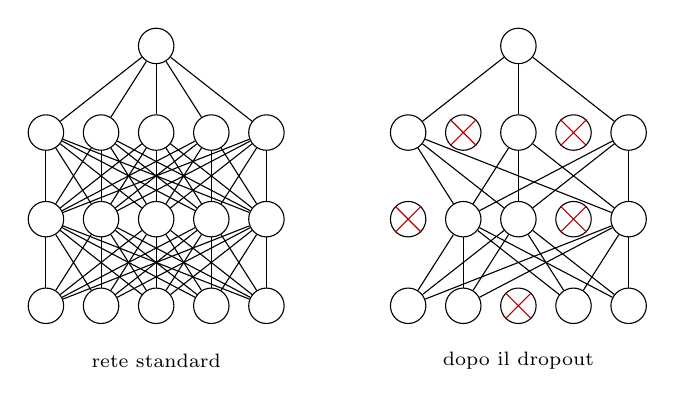
\begin{tikzpicture}[font=\scriptsize, unit/.style={draw, circle, minimum size=4.5mm, inner sep=0pt}]
  % \actA, \actB, \actC: neuroni attivi di input, primo e secondo hidden layer nella rete assottigliata
  \def\actA{1,2,4,5}
  \def\actB{2,3,5}
  \def\actC{1,3,5}
  \foreach \px/\thin in {0/0, 4.6/1} {
    \begin{scope}[shift={(\px,0)}]
      \foreach \l in {0,1,2} \foreach \i in {1,...,5}
        \node[unit] (n\l-\i) at ({0.7*(\i-1)},{1.1*\l}) {};
      \node[unit] (out) at (1.4,3.3) {};
      \ifnum\thin=0
        \foreach \i in {1,...,5} {
          \foreach \j in {1,...,5} {
            \draw (n0-\i) -- (n1-\j);
            \draw (n1-\i) -- (n2-\j);
          }
          \draw (n2-\i) -- (out);
        }
        \node at (1.4,-0.7) {rete standard};
      \else
        \foreach \i in \actA \foreach \j in \actB \draw (n0-\i) -- (n1-\j);
        \foreach \i in \actB \foreach \j in \actC \draw (n1-\i) -- (n2-\j);
        \foreach \i in \actC \draw (n2-\i) -- (out);
        \foreach \l/\i in {0/3, 1/1, 1/4, 2/2, 2/4}
          \draw[red!70!black] (n\l-\i.north west) -- (n\l-\i.south east) (n\l-\i.north east) -- (n\l-\i.south west);
        \node at (1.4,-0.7) {dopo il dropout};
      \fi
    \end{scope}
  }
\end{tikzpicture}
\end{widget}
\caption{Dropout (da \cite{Srivastava2014}). A sinistra, una rete standard con due hidden layer. A destra, una rete assottigliata ottenuta applicando il dropout alla rete di sinistra: i neuroni barrati sono stati spenti, insieme alle loro connessioni.}
\label{fig:dropout}
\end{figure}

\section{Batch normalization}
La \textbf{batch normalization} \cite{Ioffe2015} normalizza l'input e gli output delle funzioni di attivazione, così da accelerare il training delle reti profonde. Dato un mini-batch $\mathcal{B} = \{x_1, \dots, x_m\}$ con i valori di un'attivazione $x$, calcoliamo:
\begin{align*}
\mu_\mathcal{B} &= \frac{1}{m}\sum_{i=1}^m x_i && \text{media del mini-batch} \\
\sigma_\mathcal{B}^2 &= \frac{1}{m}\sum_{i=1}^m (x_i - \mu_\mathcal{B})^2 && \text{varianza del mini-batch} \\
\hat{x}_i &= \frac{x_i - \mu_\mathcal{B}}{\sqrt{\sigma_\mathcal{B}^2 + \epsilon}} && \text{normalizzazione} \\
y_i &= \gamma \hat{x}_i + \beta \equiv \mathrm{BN}_{\gamma, \beta}(x_i) && \text{scale and shift}
\end{align*}
dove $\epsilon$ è una piccola costante che evita la divisione per zero, mentre $\gamma$ e $\beta$ sono parametri appresi insieme agli altri pesi della rete. Grazie a $\gamma$ e $\beta$ la rete può riscalare e traslare le attivazioni normalizzate, e se serve può anche annullare la normalizzazione.

In fase di test non c'è un mini-batch su cui calcolare media e varianza. Si usano quindi la media e la varianza stimate sull'intero training set, calcolate come medie su più mini-batch.

La batch normalization ha due vantaggi:
\begin{itemize}
    \item \textbf{si possono usare learning rate più alti}, perché la normalizzazione evita che qualche attivazione diventi troppo grande o troppo piccola. Il training è quindi più veloce.
    \item \textbf{riduce l'overfitting}, perché ha un leggero effetto di regolarizzazione: come il dropout, aggiunge un po' di rumore alle attivazioni di ogni hidden layer.
\end{itemize}
Con la batch normalization possiamo quindi usare meno dropout, e perdere meno informazione. Tuttavia non conviene affidarsi solo alla batch normalization per la regolarizzazione: è meglio usarla insieme al dropout.

\section{Data augmentation}
La \textbf{data augmentation} è anch'essa uno schema di regolarizzazione. L'idea è aumentare la varianza dei pattern del training set generando nuovi esempi a partire da quelli che abbiamo. Si applicano trasformazioni affini ai dati di training: per ogni immagine di input si crea un ``duplicato'' traslato, ingrandito o rimpicciolito, ruotato, ribaltato, distorto o con una tonalità di colore diversa. L'immagine originale e il duplicato entrano nella rete con la stessa etichetta.

Torniamo al nostro esempio di MNIST (figura~\ref{fig:augmentation}). Da un'unica immagine di un 4 possiamo ottenere diversi esempi, tutti etichettati come 4. Le trasformazioni vanno però scelte in modo opportuno: un 4 ribaltato orizzontalmente non è più una cifra valida, mentre per la foto di un animale il ribaltamento orizzontale va benissimo. In letteratura sono stati proposti anche altri schemi di augmentation, più sofisticati.

\begin{figure}[htbp]
\centering
\begin{tikzpicture}[font=\scriptsize]
  % \cella{x}{opzioni del nodo}{larghezza dell'immagine}{didascalia}: immagine ritagliata in un riquadro nero di 1.4cm
  \def\cella#1#2#3#4{%
    \begin{scope}[shift={(#1,0)}]
      \fill[black] (-0.7,-0.7) rectangle (0.7,0.7);
      \begin{scope}
        \clip (-0.7,-0.7) rectangle (0.7,0.7);
        \node[inner sep=0pt, #2] at (0,0) {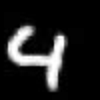
\includegraphics[width=#3]{images/mnist-4.png}};
      \end{scope}
      \node at (0,-1.0) {#4};
    \end{scope}
  }
  \cella{0}{}{1.4cm}{originale}
  \cella{1.8}{rotate=20}{1.4cm}{rotazione}
  \cella{3.6}{rotate=-20}{1.4cm}{rotazione}
  \cella{5.4}{}{2.0cm}{zoom}
  \cella{7.2}{xshift=0.3cm, yshift=-0.2cm}{1.4cm}{traslazione}
\end{tikzpicture}
\caption{Data augmentation su un'immagine di MNIST. Dall'immagine originale otteniamo nuovi esempi con rotazioni, zoom e traslazioni, che entrano nella rete con la stessa etichetta.}
\label{fig:augmentation}
\end{figure}

\section{Transfer learning}
Addestrare una rete profonda \emph{from scratch}, ovvero partendo da pesi inizializzati in modo casuale, è difficile, perché è raro avere un dataset abbastanza grande. Di solito, quindi, si parte da una rete \textbf{pre-addestrata} su un dataset molto grande (ad esempio ImageNet, EPIC-Kitchens o Ego4D). La rete viene poi usata come inizializzazione, oppure come feature extractor fisso, per il task che ci interessa. Questa idea si chiama \textbf{transfer learning}: si riutilizzano le informazioni (soprattutto quelle di basso livello) apprese da una rete per estrarre feature su un problema diverso.

Le strategie principali sono tre (figura~\ref{fig:transfer}).

\paragraph{Fixed feature extractor.}
Prendiamo un modello pre-addestrato su un task (ad esempio object recognition), rimuoviamo l'ultimo layer fully connected e usiamo il resto della rete come feature extractor fisso per il nuovo dataset. Una volta estratte le feature dal nuovo dataset, addestriamo su di esse un classificatore, ad esempio un softmax. I parametri della rete originale restano fissi durante il training del classificatore. Come classificatore si può usare anche un metodo basato sulle distanze, come il KNN che vedremo nel capitolo~\ref{ch:metric-learning}.

\paragraph{Fine-tuning.}
Sostituiamo e riaddestriamo il classificatore sul nuovo dataset, ma aggiorniamo anche i pesi della rete pre-addestrata continuando la backpropagation. Si possono aggiornare tutti i layer, oppure tenere fissi i primi (per evitare l'overfitting) e aggiornare solo la parte più alta della rete. In pratica, con il nostro dataset addestriamo gli ultimi $k$ layer, e la backpropagation aggiorna solo i loro parametri.

Perché tenere fissi i primi layer? I primi layer di una rete profonda contengono feature generiche, come rilevatori di bordi (\emph{edge detector}) o di macchie di colore (\emph{color blob detector}), utili per molti task. I layer successivi, invece, diventano via via più specifici per le classi del dataset originale.

\paragraph{Modelli pre-addestrati.}
I ricercatori rilasciano spesso i \emph{checkpoint} finali dei loro modelli, in modo che altri possano usarli per il fine-tuning. Ad esempio, la libreria PyTorch ha un sotto-pacchetto (\texttt{torchvision.models}) con le definizioni di diverse architetture e i relativi pesi.

\begin{figure}[htbp]
\centering
\begin{tikzpicture}[>=Stealth, font=\scriptsize,
  conv/.style={draw, minimum width=5mm, minimum height=1.0cm, inner sep=1pt},
  fisso/.style={fill=TextGray!25},
  nuovo/.style={draw=ObsColor, fill=ObsColor!30}]
  % \riga{y}{ultimo layer fisso}{titolo}{stile}: rete pre-addestrata, i layer da 1 a #2 hanno lo stile #4 e i successivi sono addestrati
  \def\riga#1#2#3#4{%
    \begin{scope}[shift={(0,#1)}]
      \node[anchor=west] at (-0.3,0.85) {#3};
      \foreach \k/\nm in {1/C_1, 2/C_2, 3/C_3, 4/C_4, 5/C_5, 6/f_6, 7/f_7} {
        \ifnum\k>#2
          \node[conv, nuovo] (b\k) at ({0.75*\k},0) {$\nm$};
        \else
          \node[conv, #4] (b\k) at ({0.75*\k},0) {$\nm$};
        \fi
      }
      \foreach \k [evaluate=\k as \kk using int(\k+1)] in {1,...,6} \draw[->] (b\k) -- (b\kk);
    \end{scope}
  }
  \riga{0}{7}{rete pre-addestrata}{fill=white}
  \node[conv, draw=LemmaColor, fill=LemmaColor!25] (f8) at (6.0,0) {$f_8$};
  \draw[->] (b7) -- (f8);
  \node[right, align=left] at (f8.east) {1000 classi\\di ImageNet};
  \riga{-2.0}{7}{fixed feature extractor}{fisso}
  \node[conv, nuovo] (g8) at (6.0,-2.0) {$f_8'$};
  \draw[->] (b7) -- (g8);
  \node[right, align=left] at (g8.east) {classi del\\nuovo task};
  \riga{-4.0}{4}{fine-tuning degli ultimi layer}{fisso}
  \node[conv, nuovo] (h8) at (6.0,-4.0) {$f_8'$};
  \draw[->] (b7) -- (h8);
  \node[right, align=left] at (h8.east) {classi del\\nuovo task};
  % legenda
  \node[conv, fisso, minimum height=3mm] (l1) at (0.75,-5.3) {};
  \node[right] at (l1.east) {pesi fissi};
  \node[conv, nuovo, minimum height=3mm] (l2) at (3.0,-5.3) {};
  \node[right] at (l2.east) {pesi addestrati sul nuovo dataset};
\end{tikzpicture}
\caption{Strategie di transfer learning a partire da una rete pre-addestrata su ImageNet. Con il fixed feature extractor si addestra solo il nuovo classificatore $f_8'$. Con il fine-tuning si addestrano anche gli ultimi layer della rete, mentre i primi restano fissi.}
\label{fig:transfer}
\end{figure}

\section{Quando conviene il fine-tuning}
La strategia da scegliere dipende da due fattori: la dimensione del nuovo dataset e quanto è simile al dataset originale su cui la rete è stata addestrata. Abbiamo quindi quattro casi (figura~\ref{fig:finetuning-casi}):
\begin{enumerate}
    \item \textbf{Dataset piccolo e simile all'originale}: fare fine-tuning di tutta la rete può portare all'overfitting. Conviene addestrare solo il layer appena aggiunto.
    \item \textbf{Dataset grande e simile all'originale}: più dati abbiamo, meglio è. Possiamo addestrare tutta la rete.
    \item \textbf{Dataset piccolo e diverso dall'originale}: addestrare tutta la rete non è una buona idea. Tuttavia il nuovo layer non va aggiunto in cima, perché gli ultimi layer sono molto specifici per il dataset (e il problema) originale. Conviene aggiungerlo a una parte precedente della rete.
    \item \textbf{Dataset grande e diverso dall'originale}: possiamo fare fine-tuning di tutta la rete. Equivale a un nuovo training, in cui però i pesi sono inizializzati con quelli di un'altra rete.
\end{enumerate}
In tutti i casi, partire da pesi pre-addestrati conviene: hanno già un senso, mentre dei pesi inizializzati in modo casuale no. Il vantaggio è massimo quando il dataset è piccolo ma simile all'originale.

\begin{figure}[htbp]
\centering
\begin{tikzpicture}[font=\scriptsize,
  caso/.style={draw, minimum width=4.4cm, minimum height=1.6cm, text width=4.1cm, align=center}]
  \node[caso, fill=LemmaColor!15] at (0,0) {\textbf{1.} addestrare solo\\il nuovo layer};
  \node[caso, fill=LemmaColor!30] at (4.4,0) {\textbf{2.} addestrare\\tutta la rete};
  \node[caso, fill=ObsColor!15] at (0,-1.6) {\textbf{3.} aggiungere il nuovo layer\\a una parte precedente della rete};
  \node[caso, fill=ObsColor!30] at (4.4,-1.6) {\textbf{4.} fine-tuning di tutta la rete\\(nuovo training con pesi pre-addestrati)};
  \node[above] at (0,0.8) {dataset piccolo};
  \node[above] at (4.4,0.8) {dataset grande};
  \node[left, align=right] at (-2.25,0) {simile\\all'originale};
  \node[left, align=right] at (-2.25,-1.6) {diverso\\dall'originale};
\end{tikzpicture}
\caption{La strategia di fine-tuning in base alla dimensione del nuovo dataset (colonne) e alla sua somiglianza con il dataset originale (righe).}
\label{fig:finetuning-casi}
\end{figure}

\section*{Riferimenti}
Il materiale visto in questo capitolo comprende:
\begin{itemize}
    \item Materiale visto a lezione (27 ottobre 2026).
    \item Slide del corso \emph{Convolutional Neural Net}, dal dropout al fine-tuning.
    \item \citetitle{Srivastava2014} \cite{Srivastava2014}, il paper originale sul dropout, da cui è tratta la figura~\ref{fig:dropout}.
    \item \citetitle{Ioffe2015} \cite{Ioffe2015}, il paper originale sulla batch normalization.
\end{itemize}
